\subsection{Session 4, Exercise 5}

\lineparagraph{Exercise}

Let the alphabet be $\Sigma=\{0,1\}$, states of the pushdown automaton be $Q=\{A,B,C\}$, where $A$ is the start state, $C$ is the only accept state, let $Z$ be the start symbol of the stack. The transition function is the following:

\begin{align*}
    1.\text{ }\delta(A,0,\varepsilon) = \{(A,a)\}\\
    2.\text{ }\delta(A,1,\varepsilon) = \{(A, b)\}\\
    3.\text{ }\delta(A,\varepsilon,\varepsilon) = \{(B,\varepsilon)\}\\
    4.\text{ }\delta(B,0,a) = \{(B,\varepsilon)\}\\
    5.\text{ }\delta(B,1,b) = \{(B,\varepsilon)\}\\
    6.\text{ }\delta(B,\varepsilon, Z) = \{(C,\varepsilon)\}
\end{align*}

\begin{enumerate}[a)]
    \item Give the possible computations of the automaton on word 010.
    \item Does it accept word 0110?
    \item What is the language recognized by the automaton?
    \item Give a CF-grammar for this language.
\end{enumerate}

\lineparagraph{Solution}

a)

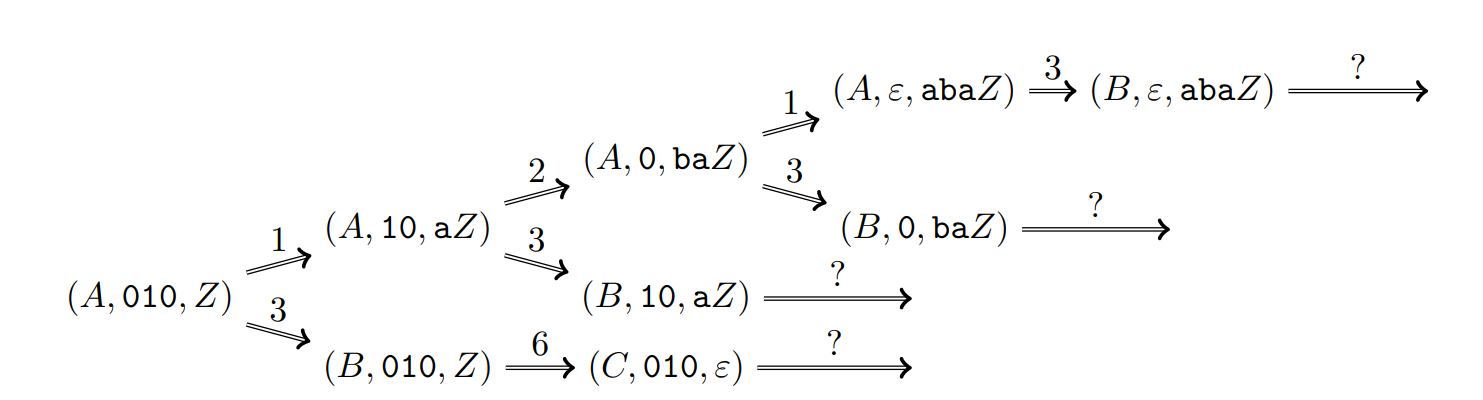
\includegraphics[width=\linewidth]{04/4_5_a.png}

b)

Yes, for example an accepting comutation (branch) is the following:


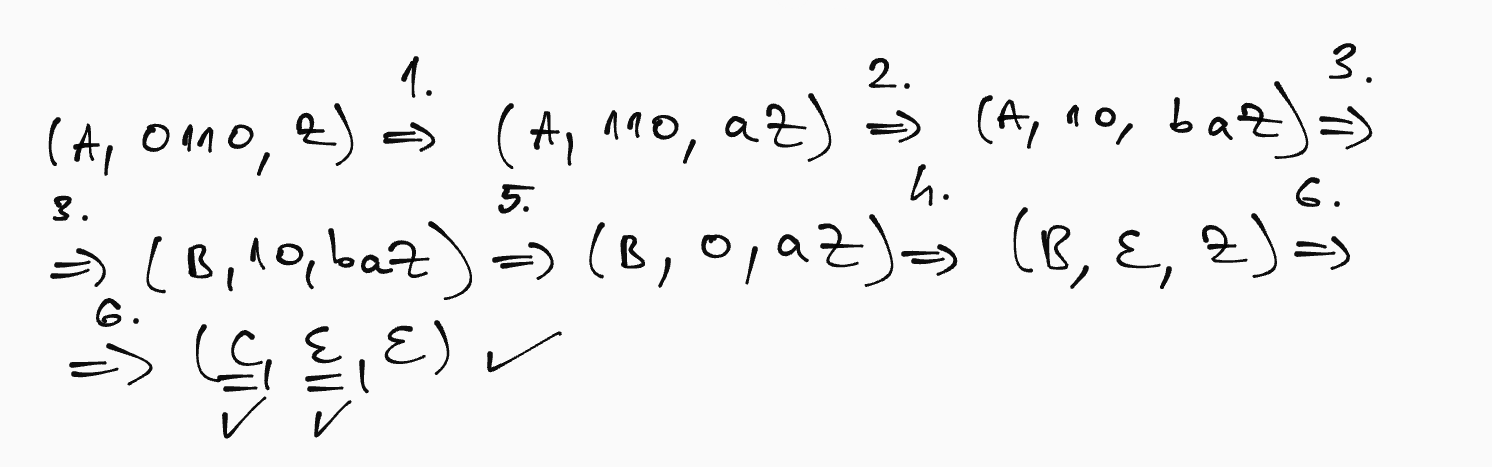
\includegraphics[width=\linewidth]{04/4_5_b.png}

c)

The language recognized is palindromes of odd length. These are accepted, since an accepting computation for these types of words will be: for the first half of the word transitions $1.$ and $2.$ will push the word ($0=a$, $1=b$) into the stack, then transition $3.$ will move to variable $B$, where the second (mirrored) half of the word will be compared to the first half on the stack using transitions $4.$ and $5.$. Since a stack is last-in-first-out, the comparisons will happen in the correct order. The stack can be emptied out this way and that allows for transition $6.$ to occur on the stack bottom symbol and move to the acceting $C$ state.

Words not in this language are rejected, since:
\begin{itemize}
    \item Only words of even length have a chance to be accepted, since the stack must be emptied out to move to the only accepting state and each character we put on the stack must have a pair that we use to remove it from the stack.
    \item Transition $3.$ must occur exactly at the middle of the word, for the same reason as stated above: if the word's length is $2n$, $n$ characters must be put on the stack, then move to state $B$, where $n$ characters must be removed from the stack. If the transition occurs too late, there will be remaining characters on the stack and we won't be able to move to state $C$, while if the transition occurs too early, the stack might be emptied out, however there will be remaining characters on he input so we could move to state $C$, however we won't accept since there are remaining characters on the input.
    \item If the word is not a palindrome, there must be at least one position where the character on it's mirrored position is wrong, either $a$ paired with a $b$ or $b$ paired with an $a$. This means, that when reading the stack back in state $B$, when we reach this position, we will have a wrong pairing: $0$ on the input with a character $b$ on the stack, or $1$ on the input with a character $a$ on the stack, for which no transition is defined from $B$, thus the machine will stop and the stack will not be empty, so we cannot move to state $C$ and $B$ is a rejecting state (plus, there will also be remaining input as well).
\end{itemize}

d)

\begin{align*}
    S \rightarrow& aSa | bSb | \varepsilon
\end{align*}

We have shown in previous exercises that this is indeed the grammar for palindromes of even length.